

\begin{figure}[h]
 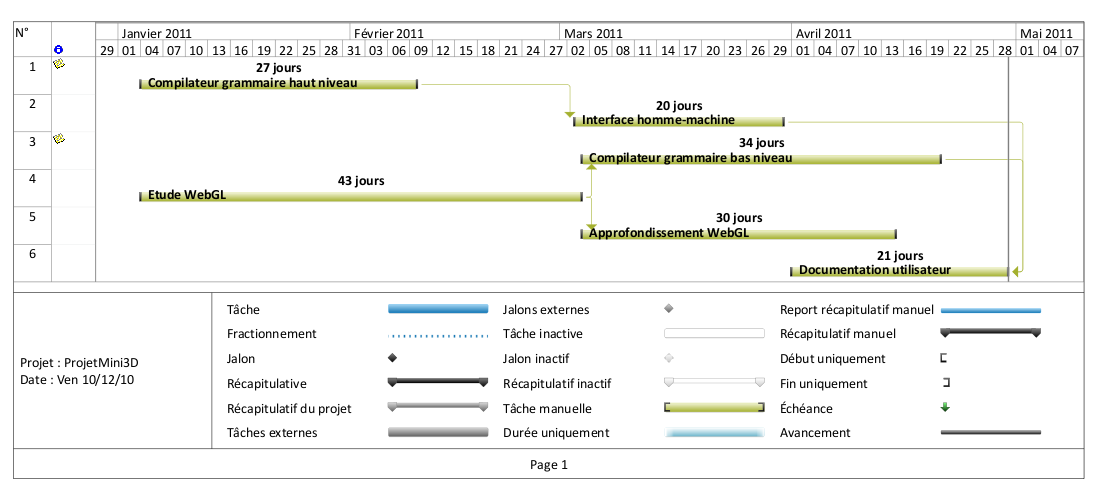
\includegraphics[width=\textwidth]{strategie/diag_gantt}
\end{figure}

\begin{figure}[h]
 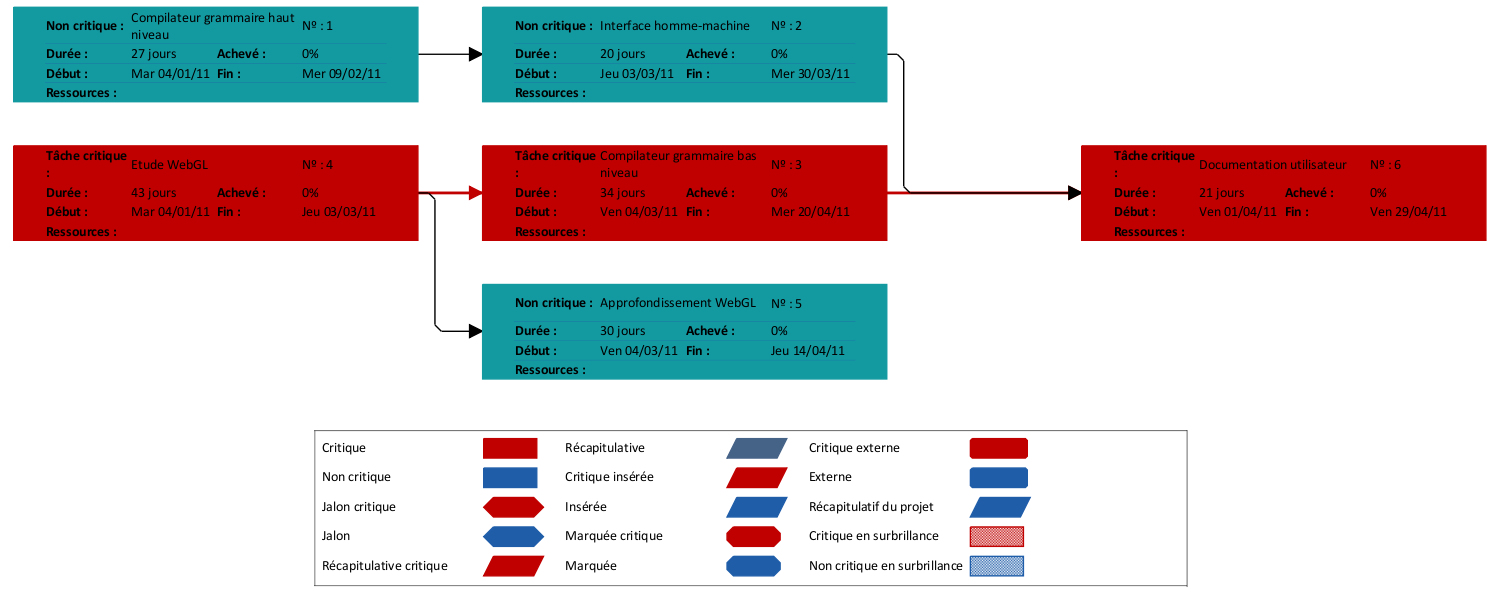
\includegraphics[width=\textwidth]{strategie/org_desc_tach}
\end{figure}

La première phase de développement se concentrera sur le compilateur du langage haut niveau qui ne nécessite pas d’apprentissage particulier 
puisque les bases du langage client (javascript) ont déjà été  étudiées lors de la phase d’analyse. 
En parallèle, sera effectuée une recherche générale sur l’utilisation de WebGL qui est un langage peu documenté car très récent, 
mais nécessaire à la suite du projet. Pour cette raison, une longue durée lui est consacrée.


WebGL incarne le principal risque du projet car nous ne savons pas le manipuler et nous ne connaissons pas ses limites.
 C’est une part d’inconnu qui pourrait potentiellement retarder le démarrage des tâches suivantes ainsi qu’affecter la bonne marche de celles 
liées au développement des compilateurs ; soit par obligation de modifier les grammaires établies pour répondre à des problèmes propres au WebGL 
soit par des difficultés d’implantation, causées par le manque de maturité du langage.

Une fois l’étude WebGL achevée, le développement du compilateur du langage bas niveau pourra commencer ainsi qu’un approfondissement de WebGL.


Lorsque les bases du compilateur du langage haut niveau seront établies, le développement de l’interface homme-machine pourra débuter.
 Un battement d’une semaine est prévu car il est fort probable que des modifications de ce compilateur aient lieu après une première finalisation.

La méthode agile répond aux besoins du projet, notamment à la souplesse qu’il demande. 
En conséquence, seront employés, le couple des méthodes Scrum et Extreme Programming. 